\documentclass[9pt,twocolumn,twoside]{../../styles/osajnl}
\usepackage{fancyvrb}
\journal{i524} 

\title{Google Fusion Table}


\author[1,2]{Milind Suryawanshi}


\affil[1]{School of Informatics and Computing, Bloomington, IN 47408, U.S.A.}
\affil[2]{Electronics and Telecommunication Engineer,Pune University, 2010}
\affil[*]{Corresponding authors: laszewski@gmail.com}

\dates{Paper-1 S17-IO-3020, \today}

\ociscodes{Fusion Tables, data, query, I524}

% replace this with your url in github/gitlab
\doi{\url{https://github.com/cloudmesh/classes/blob/master/docs/source/format/report/report.pdf}}


\begin{abstract}
Fusion Table is a web service provided by Google. It is a data management tool, which provides the features data gathering, storing data in tables, visualizing stored data, merging tables, sharing table, view and download the tables. 
\newline
\end{abstract}

\setboolean{displaycopyright}{true}

\begin{document}

\maketitle

\section{Introduction}

Fusion Table is a “cloud Software as a Service (SaaS) application” \cite{www-1}. It’s a data visualization web application, which gathers, stored, share and visualize data. User can store data in tables and can represent it in the form of different charts, maps and plots. This information can be share, merged, published by individual user or website.  

 
Fusion table provides capacity to import tables/files up to 250MB \cite{www-2} of the type csv (Comma Separated Value), tsv (text-delimited files), kml (KML), spreadsheets (e.g. xls, xsls, ods) and google spreadsheet. Google provides quota of 1 GB per user to store tables. This 1 GB limit does not count the shared tables and tables in trash as a user quota \cite{www-2}. Fusion table helps to visualize the stored data in unambiguous chart format, like: pie charts, bar charts, line plots, scatterplots, timelines and the geographical maps are provided. Fusion Tables service got launched in June 9 2009, and added to the Google Docs feature in 2011 \cite{www-3}. Now they have released the v2 (version-2) of fusion table and v1 (version-1) has been deprecated from May 3rd, 2016 and be available till August 1st, 2017 \cite{www-4}.


Fusion tables uses HTTP request to perform the various tasks on tables. It allows users to \cite{www-5}:

\begin{itemize}
	\item create and delete tables
	\item read and modify the table column name and type
	\item insert, update and delete the rows in a table.
	\item Can change the access control of certain tables and its visualization.
	\item Fire quires on row to perform required tasks.
\end{itemize}

Data operation on table are performed through subset of SQL queries using HTTP request, also it used for retrieve the tables either in CSV or JSON file format. It uses the JSON format to make the changes in default behavior of table structure, metadata and visualization settings \cite{www-5}. 



\section{Architecture}

Fig-1 shows the architecture of Fusion Table; we are discussing the architecture component of Fusion Table. Which explains the storage stack, Bigtable and user table schema information. 
 

\begin{figure}[htbp]
	\centering
	\fbox{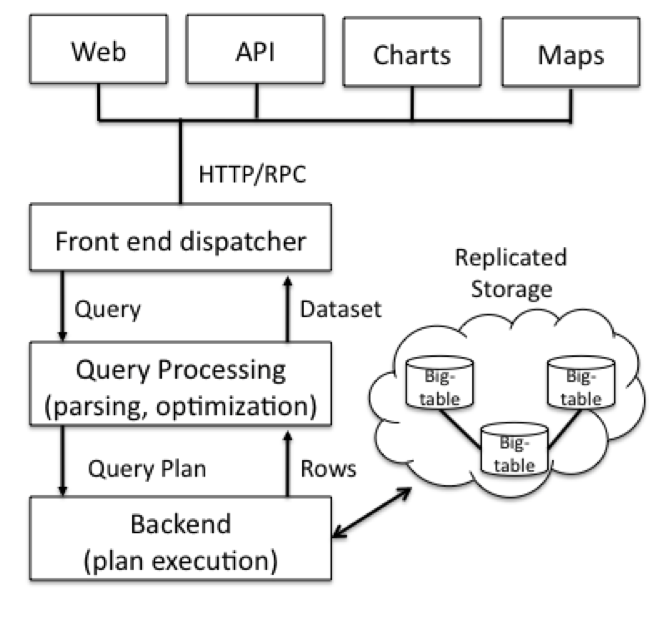
\includegraphics[width=\linewidth]{images/arch}}
	\caption{Fusion Table Architecture }
	\label{fig:false-color}
\end{figure}

The service request in Fusion table is generated through Web, API, Charts and Maps. Web is a Fusion Table website, API will be from app which provides Fusion Table services, Charts to visualize the chart and to use spatial, the Maps service being used. These service request gets handled by the front end dispatcher. It will convert the above service request into required format and passes it to Query Processing. Front end dispatcher receives the dataset from Query Processing. The Query Processing convert the query into query plan. Here the query will be getting parsed and optimize to enhance the response of a query. Then Backend module’s will execute the query plan received form Query Processing. Backend module will be responsible for fetching the diverse data of different table, sizes and queries from Storage. Also provides the requested (through optimize queries) data in rows \cite{www-6}.



\section{Storage System}

Fusion Table provide large data storage capacity, it internally uses two-layer data storage, Bigtable and Magastore. It known as Google storage stack.

\textbf{Bigtable:} Bigtable stores data in tuples (it’s a row, in a context of database ), in key-value pair form. Its also stores the transaction timestamp history, the timestamp is a time when the tuples get written in table. Bigtable sorts the keys and stores the shard key in respective servers, according the key. Bigtable performs read and write operation. Write operation done automatically where read operation can be performed in 3 forms. Read by key prefix, read by key range or read key by exact key. 

\textbf{Megastore:}  It is “library on top of Bigtable” \cite{www-6}. Megastore provide higher level operation like consistent secondary indexes, multi-row transaction and consistent replication.

\textbf{Row Store:} Fusion table stores all users table in to a single table called Rows, this being possible by Bigtable. Users table row gets saved in a table with key of a row with id of user’s table. If a new user adds a table, then Bigtable splits the Rows table into sub-tables. Now this sub-tables are handled by separate server, which provide good performance in querying millions of tables. Bitables stored the property value of table in string format. Please see table 1.1.

\begin{figure}[htbp]
	\centering
	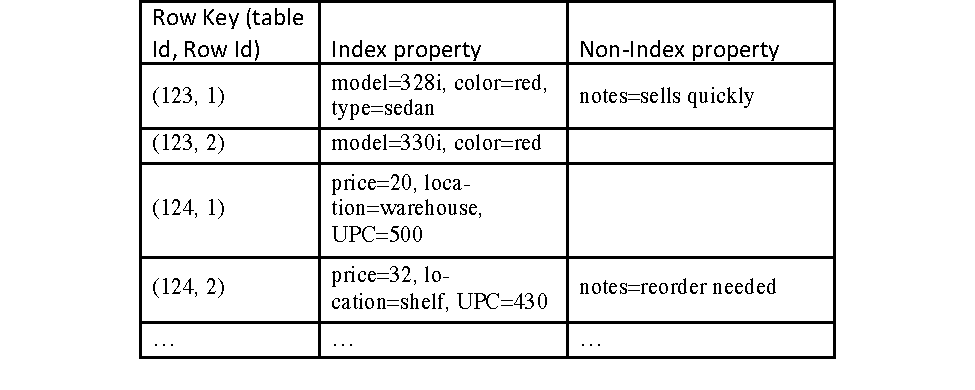
\includegraphics[width=\linewidth]{images/table1}
	\caption{As an example of sub-table}
	\label{fig:false-color}
\end{figure}


Observe the above table, it’s a subset of Rows table. It holds the values for two different table, table 123, and 124, with its row Id e.g.1, 2. If we observe the row of table 123, with row id-1 holds the property model, color, type and notes. Where row-2 holds the value of model and color.

\section{Query Processing}

As mentioned above, Fusion Table uses Bigtable and MegaStore for storage, and it useless subset of SQL, for query processing. In Fusion table we use different kind of queries to retrieve the results, following are the few common queries:

\textbf{Prefix scan:} This is the query type with prefix value. E.g. “select * from 111 limit 50”.  Here the result rows would be with prefix value = 111 up to the count 50;

\textbf{Index prefix scan:} Here the scan would be performing on index and the prefix value. E.g. “select * from 111 where color = ‘blue’”. This query will result the rows with prefix value 111 and the color is blue. 

\textbf{Index range scan:} The queries which provides the result in range. E.g. “select * from 111 where price 10 and price 20”. The query will result in rows, which have the prefix 111 and has the price in the range of 10 to 20.

\textbf{Index join:} Such queries particularly used in merging the table. It either merges the small table into big one or do the index merging. Parallel query will prefix the keys (in this example A.key and B.key) and compare the matching rows, such pairs then retrieved from the rows table. Query example: “select * from A.key = B.key”.  




\section{Visualization feature}

Google provide powerful collection of visualization frameworks \cite{www-7}. Which provides API to embed in website to show the real time data. 
Where the user can integrate the visualization in the website with data, which will show the refection of data changes directly in the graph/maps. It provides data set interface to obtain data, for visualization \cite{www-7}. 


Fusion tables facilitate the integration of geo location in website as well. Where user can upload a table with street address, points, lines or polygons. This data then rendered on server side and that will send to the user’s website where it has been integrated, in the form of tiles (images). Following is the example of map service integration using Fusion Table.


\begin{figure}[htbp]
	\centering
	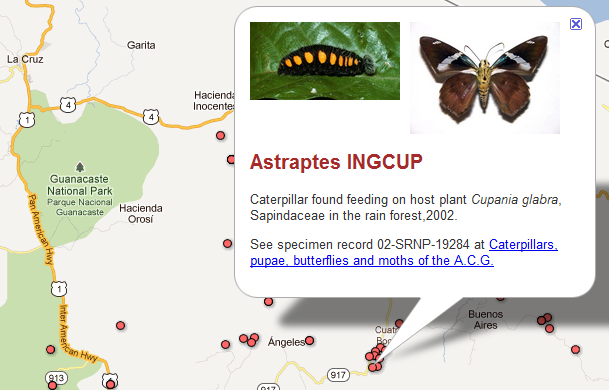
\includegraphics[width=\linewidth]{images/ft_mapresult}
	\caption{Map service integration using Fusion Table \cite{www-8} }
	\label{fig:false-color}
\end{figure}


Like the maps, user can also integrate the pie charts, line charts, bar carts, scatter chart as per the requirement . 


\section{Latest Features}

\begin{enumerate}
	\item Controlled sharing of data, user can share the specific data which should be shared with other user.
	\item Chart tooltip layout: Shows the information about the values after one would hover over them.
	\item Filtering option: “NOT” queries and regular expression matching. 
	\item Custom table and column properties.
	\item Extended quota limits up to 1GB per user, and user can store 250 MB data per table.
	\item Media download of large tables: provide large tables download facility without having server timeout problem.

\end{enumerate}


\section{Conclusion}

Google Fusion Tables is a web application used for sharing, visualizing and publishing of data on websites. It is also known as SaaS app, hosted and maintained by Google cloud services. This service can be accessible to user through Internet (using browser) or by using application. User can upload files (CSV, KML, ODS, XLS or Google Spreadsheet) to the Fusion Tables table. This data can be then visualize using different kind of charts, for private use or embed in website. Fusion Tables table can be used for real time data changes and its reflection on charts/map. As in collaboration of all the feature, Fusion table is helpful in data management tool and data analytics operation, with good scalability. Also it provides a real time data collaboration with add, delete, edit and comment feature to the users. Integration to Google will provide our tables, maps are searchable to Google’s crawlers.  


\section{Acknowledgement}


Thanks to Professor Gregor von Laszewski for giving me an opportunity and encouragement to create a technical paper.
Also the entire class and TA's for their suggestion for paper.

% Bibliography

\bibliography{references}
 


\end{document}
